\documentclass[dvipdfmx,autodetect-engine,titlepage]{jsarticle}
\usepackage[dvipdfm]{graphicx}
\usepackage{ascmac}
\usepackage{fancybox}
\usepackage{listings}
\usepackage{plistings}
\usepackage{itembkbx}
\usepackage{amsmath}
\usepackage{url}
\usepackage{graphics}
\usepackage{listings}
\usepackage{here}

\lstset{%
  language={C},
  basicstyle={\small},%
  identifierstyle={\small},%
  commentstyle={\small\itshape\color[rgb]{0,0.5,0}},%
  keywordstyle={\small\bfseries\color[rgb]{0,0,1}},%
  ndkeywordstyle={\small},%
  stringstyle={\small\ttfamily\color[rgb]{1,0,1}},
  frame={tb},
  breaklines=true,
  columns=[l]{fullflexible},%
  numbers=left,%
  xrightmargin=0zw,%
  xleftmargin=3zw,%
  numberstyle={\scriptsize},%
  stepnumber=1,
  numbersep=1zw,%
  lineskip=-0.5ex%
}

\textheight=23cm
\renewcommand{\figurename}{図}
\renewcommand{\tablename}{表}
\newenvironment{code}
{\vspace{0.5zw}\VerbatimEnvironment  \begin{screen} 
\baselineskip=1.0\normalbaselineskip
 \begin{Verbatim}}
{\end{Verbatim}
\baselineskip=\normalbaselineskip
 \end{screen}\vspace{0.5zw}} 

\title{自然言語処理(R)\\
第5回レポート\\
}
\author{26002000872\\Oku Wakana\\奥 若菜}
\date{May. 20 2022}

\begin{document}

\maketitle

\section{課題内容}
与えられた日本語文法を用いて「ヒロシが病院でもらった薬を飲んだ」という文章を句構造解析する。\\\\

\section{CYK法を用いた構文解析表の作成}
与えられた文章にCYKアルゴリズムを適用し、下の図1のような構文解析表を作成した。\\

 \begin{figure}[H]
    \centering
    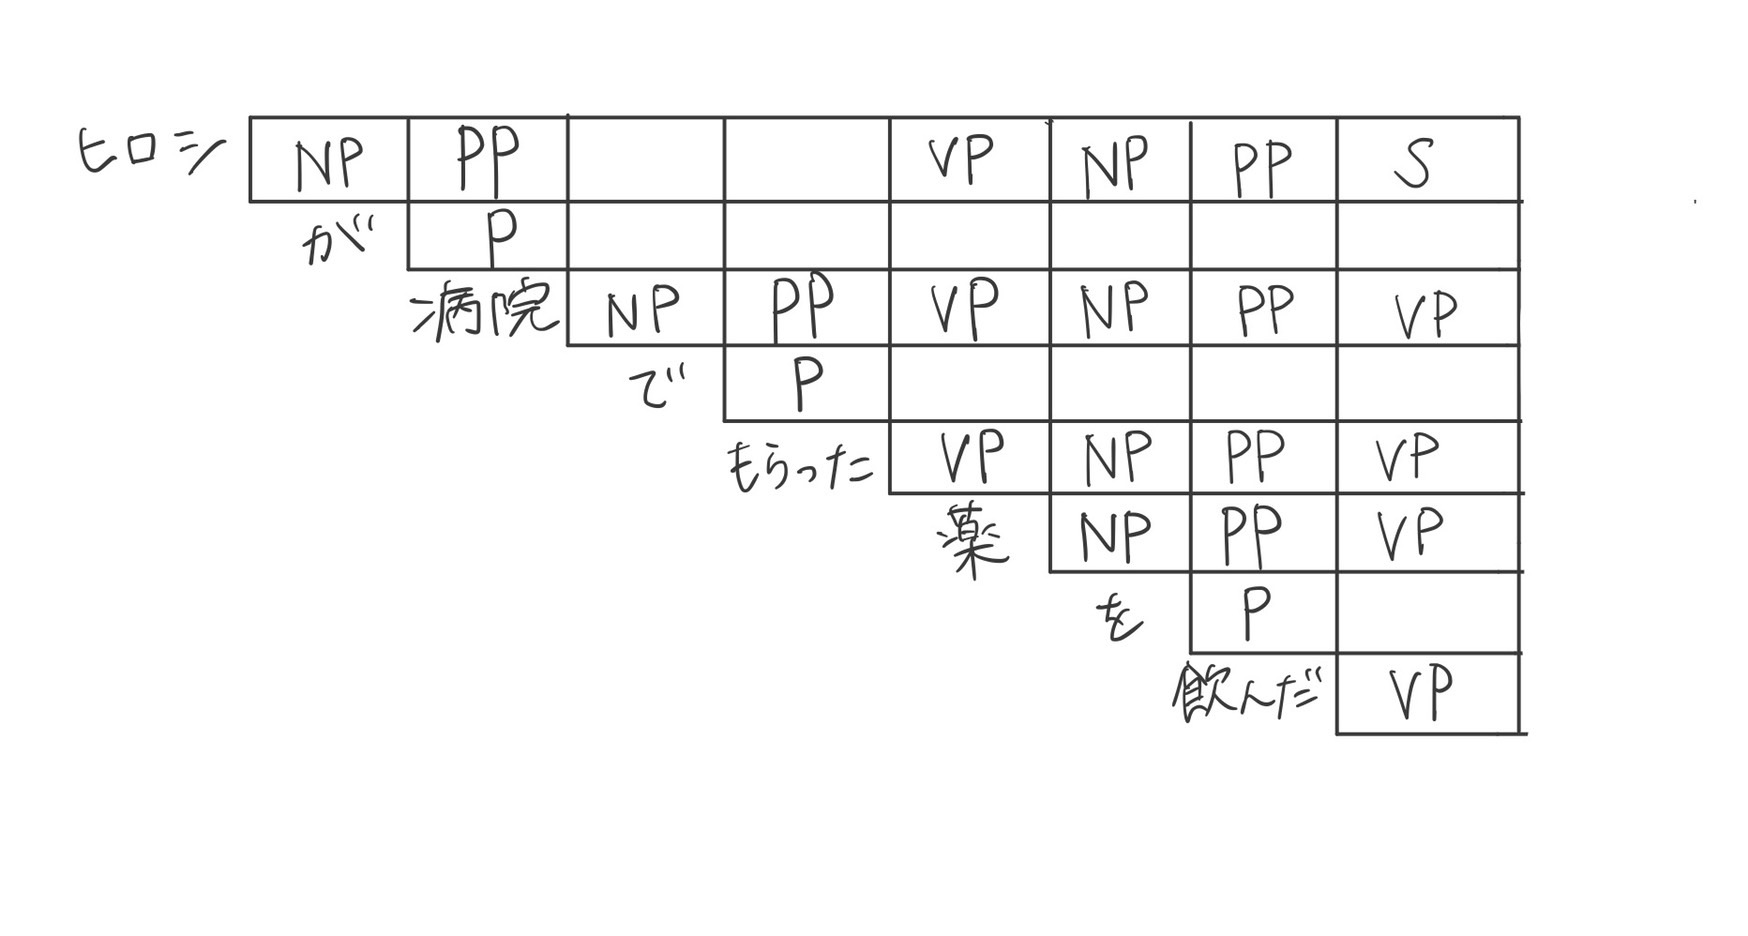
\includegraphics[scale=0.2]{s1.jpg}
    \caption{CYK構文解析表}\label{fig:図}
\end{figure}

\section{構文木の作成過程}
構文解析表から、与えられた文章の句構造を表すための構文木を作成する。図1の構文解析表からは以下の図2,3,4に示す3通りのルートが得られた。\\

 \begin{figure}[H]
    \centering
    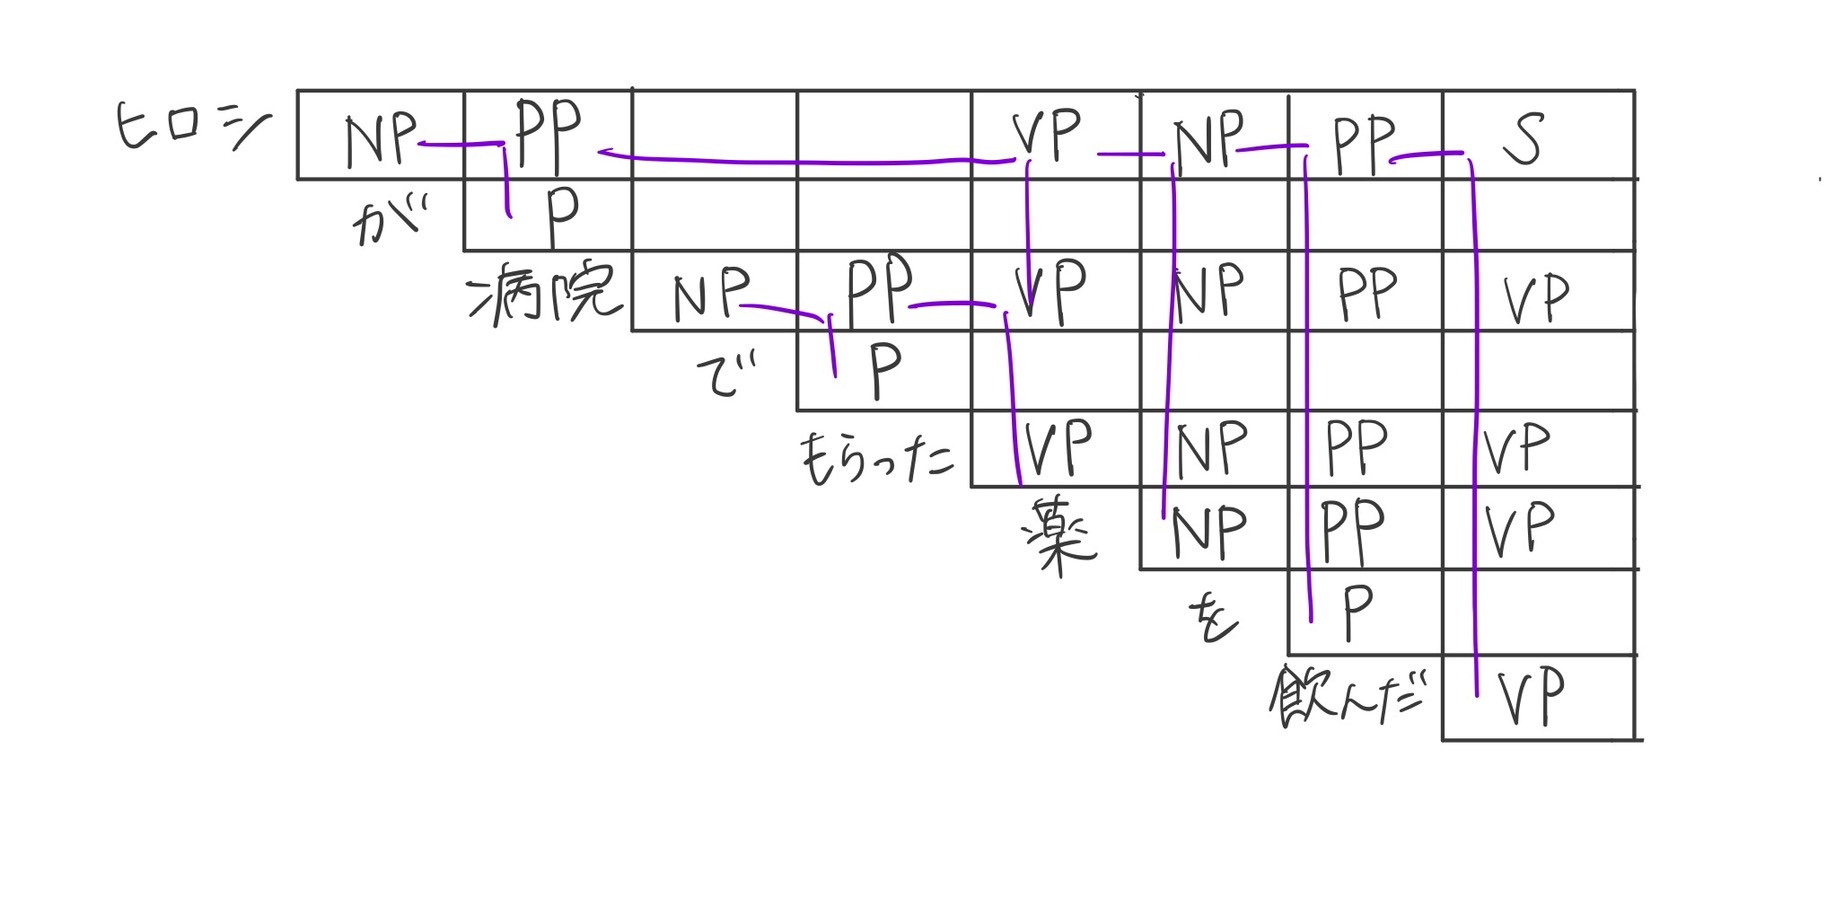
\includegraphics[scale=0.17]{s2.jpg}
    \caption{ルート1}\label{fig:図}
\end{figure}

 \begin{figure}[H]
    \centering
    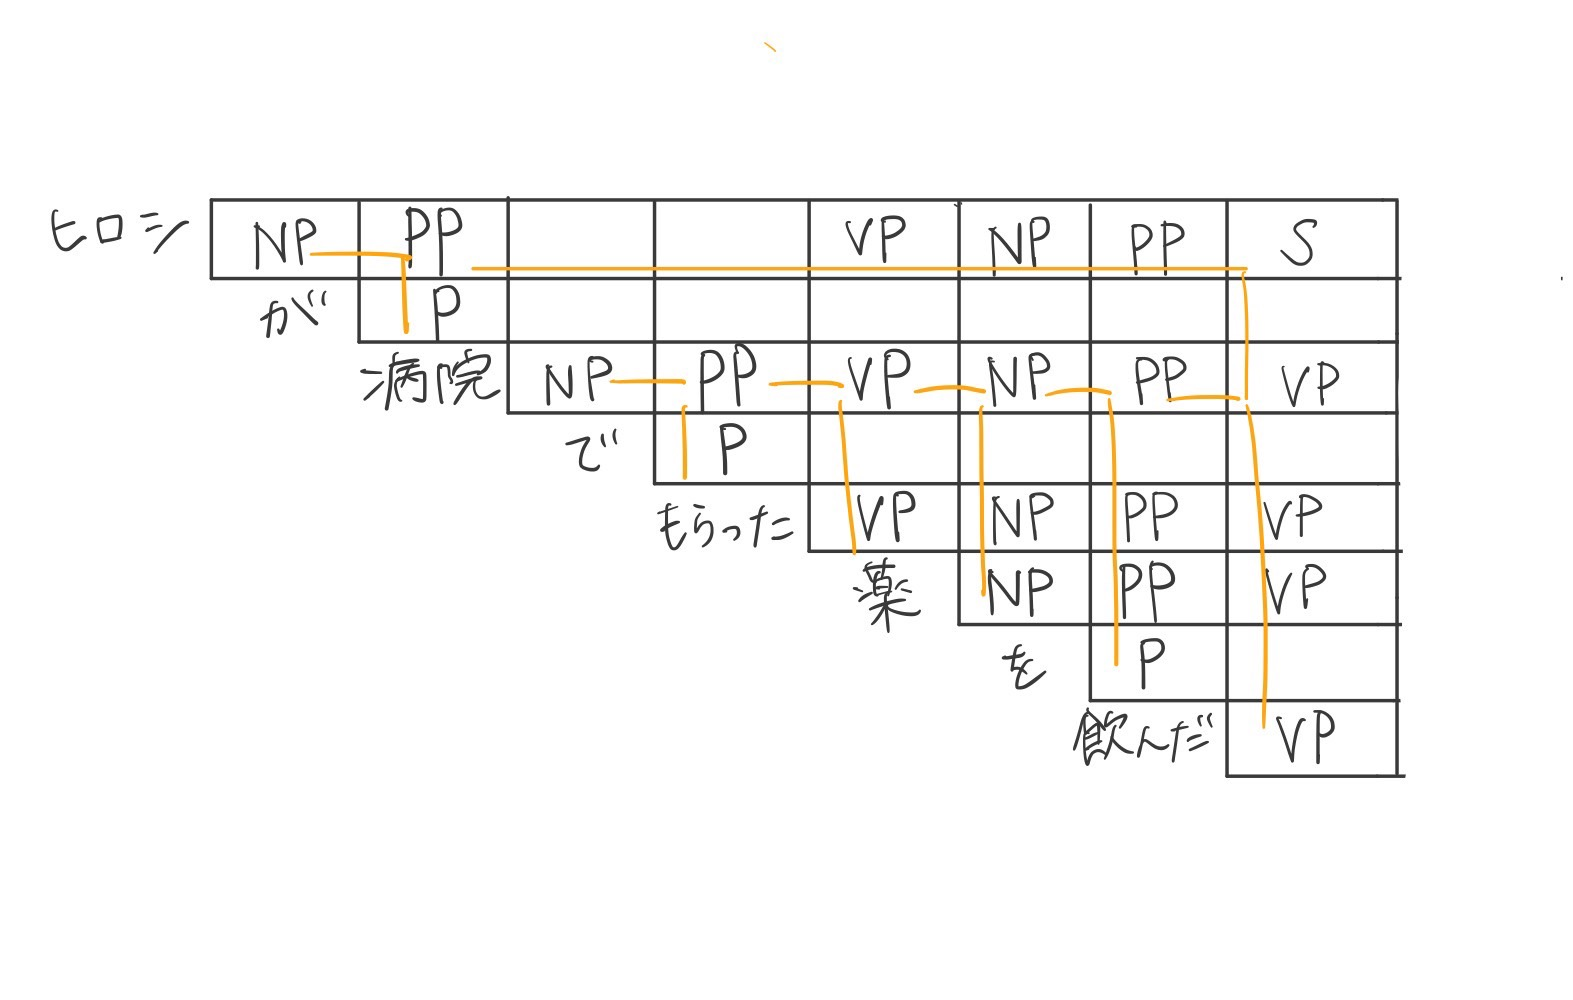
\includegraphics[scale=0.17]{s3.jpg}
    \caption{ルート2}\label{fig:図}
\end{figure}

 \begin{figure}[H]
    \centering
    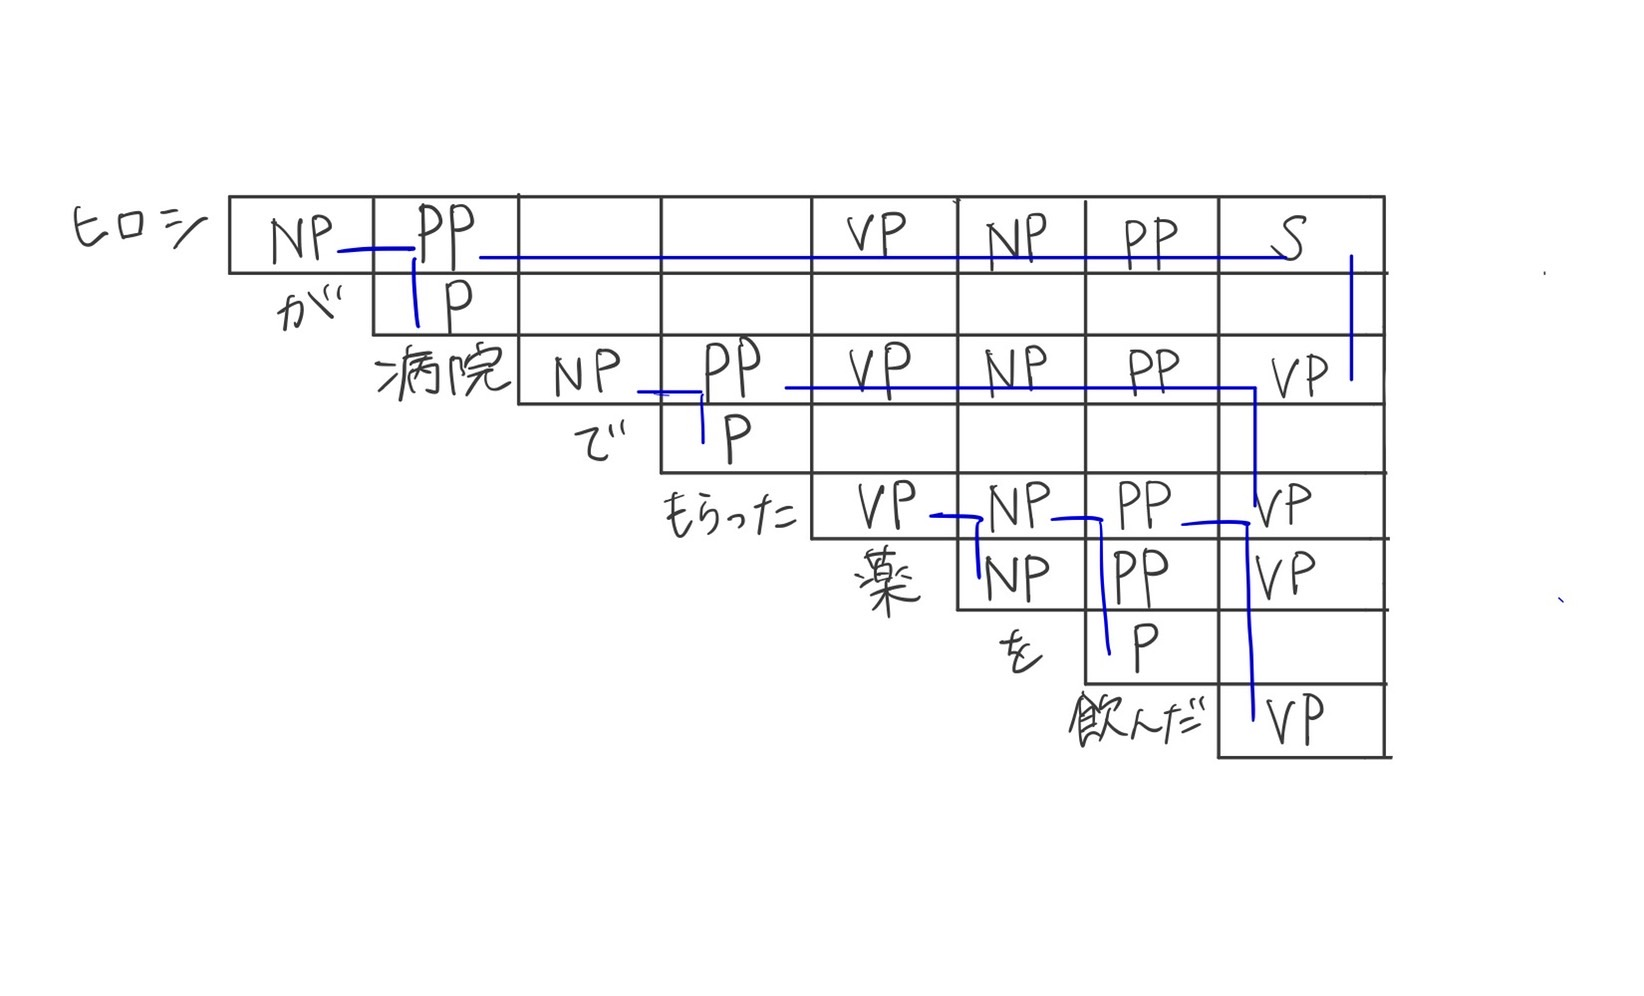
\includegraphics[scale=0.17]{s4.jpg}
    \caption{ルート3}\label{fig:図}
\end{figure}

\section{結果}
図2,3,4を構文木に直したものが下の図5,6,7であり、これらが今回の句構造解析によって得られた全ての句構造である。\\


\begin{figure}[h]
  \centering
  \begin{minipage}[b]{0.45\linewidth}
  \begin{center}
    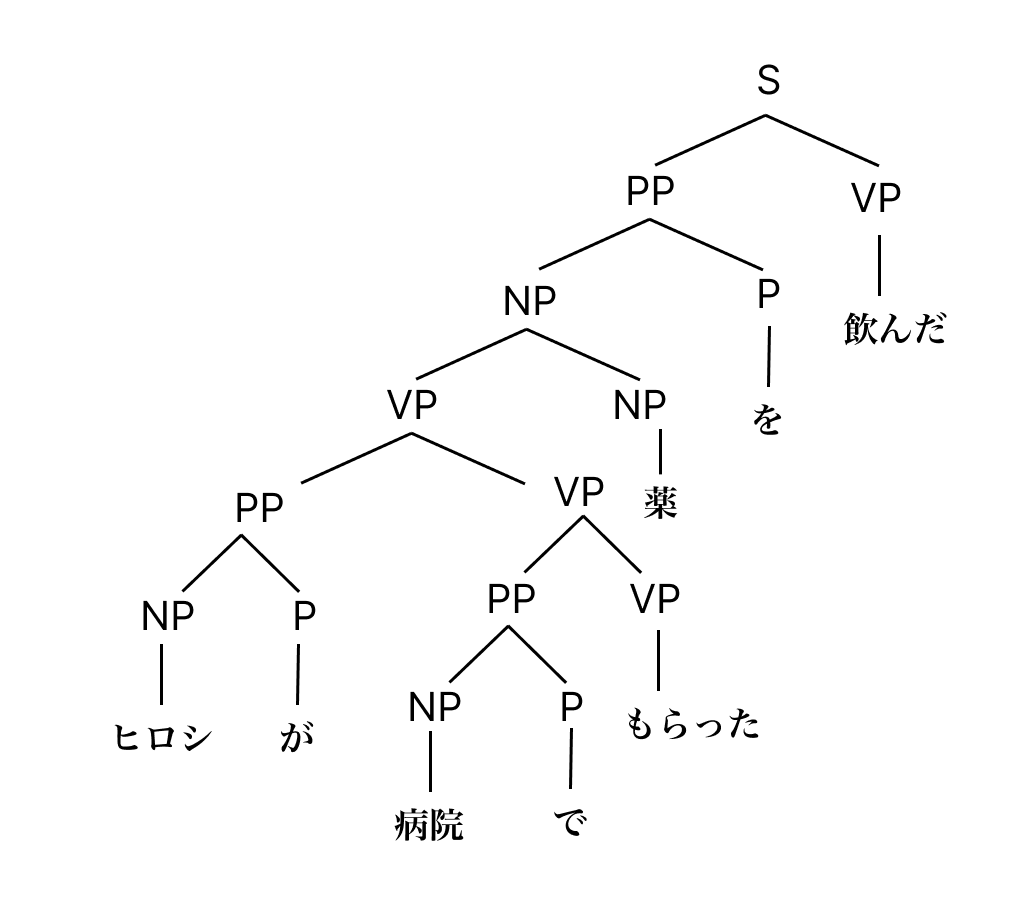
\includegraphics[keepaspectratio,scale=0.18]{tree1.png}
    \end{center}
    \caption{構文木1}
  \end{minipage}
  \begin{minipage}[b]{0.45\linewidth}
  \begin{center}
    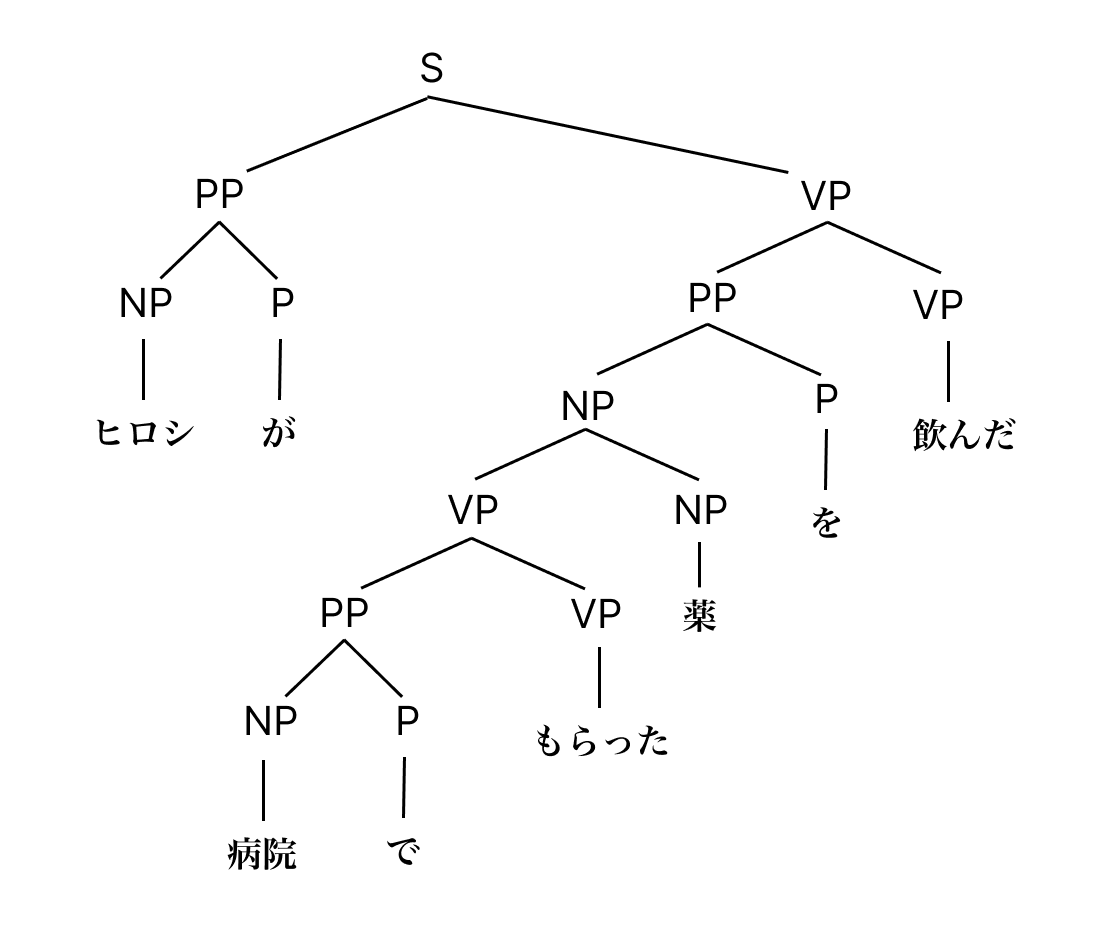
\includegraphics[keepaspectratio,scale=0.18]{tree2.png}
    \end{center}
    \caption{構文木2}
  \end{minipage}
\end{figure}

 \begin{figure}[H]
    \centering
    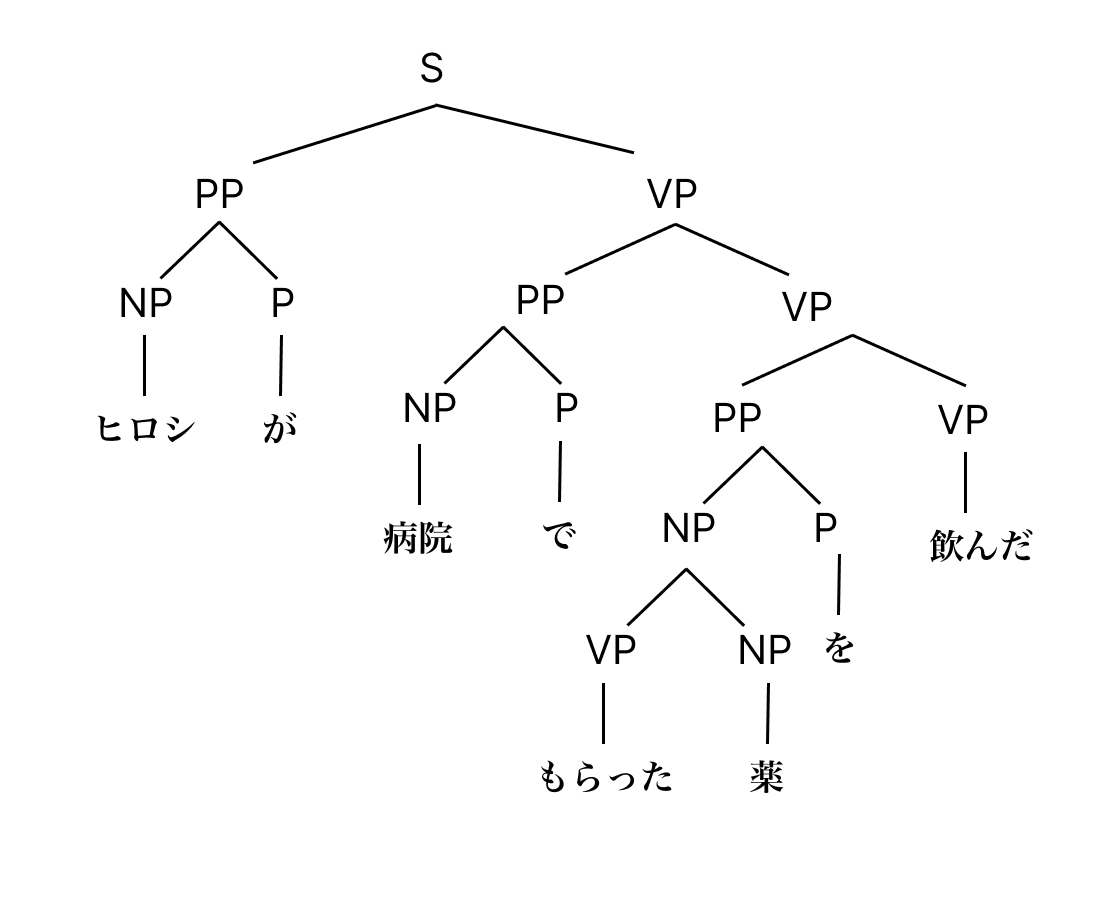
\includegraphics[scale=0.17]{tree3.png}
    \caption{構文木3}\label{fig:図}
\end{figure}



\end{document}

\lstset{%
  language={C},
  basicstyle={\small},%
  identifierstyle={\small},%
  commentstyle={\small\itshape\color[rgb]{0,0.5,0}},%
  keywordstyle={\small\bfseries\color[rgb]{0,0,1}},%
  ndkeywordstyle={\small},%
  stringstyle={\small\ttfamily\color[rgb]{1,0,1}},
  frame={tb},
  breaklines=true,
  columns=[l]{fullflexible},%
  numbers=left,%
  xrightmargin=0zw,%
  xleftmargin=3zw,%
  numberstyle={\scriptsize},%
  stepnumber=1,
  numbersep=1zw,%
  lineskip=-0.5ex%
}

\textheight=23cm
\renewcommand{\figurename}{図}
\renewcommand{\tablename}{表}
\newenvironment{code}
{\vspace{0.5zw}\VerbatimEnvironment  \begin{screen} 
\baselineskip=1.0\normalbaselineskip
 \begin{Verbatim}}
{\end{Verbatim}
\baselineskip=\normalbaselineskip
 \end{screen}\vspace{0.5zw}} 

\title{自然言語処理(R)\\
第5回レポート\\
}
\author{26002000872\\Oku Wakana\\奥 若菜}
\date{May. 14 2022}

\begin{document}

\maketitle

\section{課題内容}
単語辞書と連接可否行列を用いて、「頭痛を飲み薬でなおした」という文章を形態素解析する。\\\\

\section{制約適用によるラティス作成}
下の図1は、形態素解析する文章の表記に部分一致する全ての単語を辞書から抜き出し、単語の候補を列挙したラティス構造である。\\

 \begin{figure}[H]
    \centering
    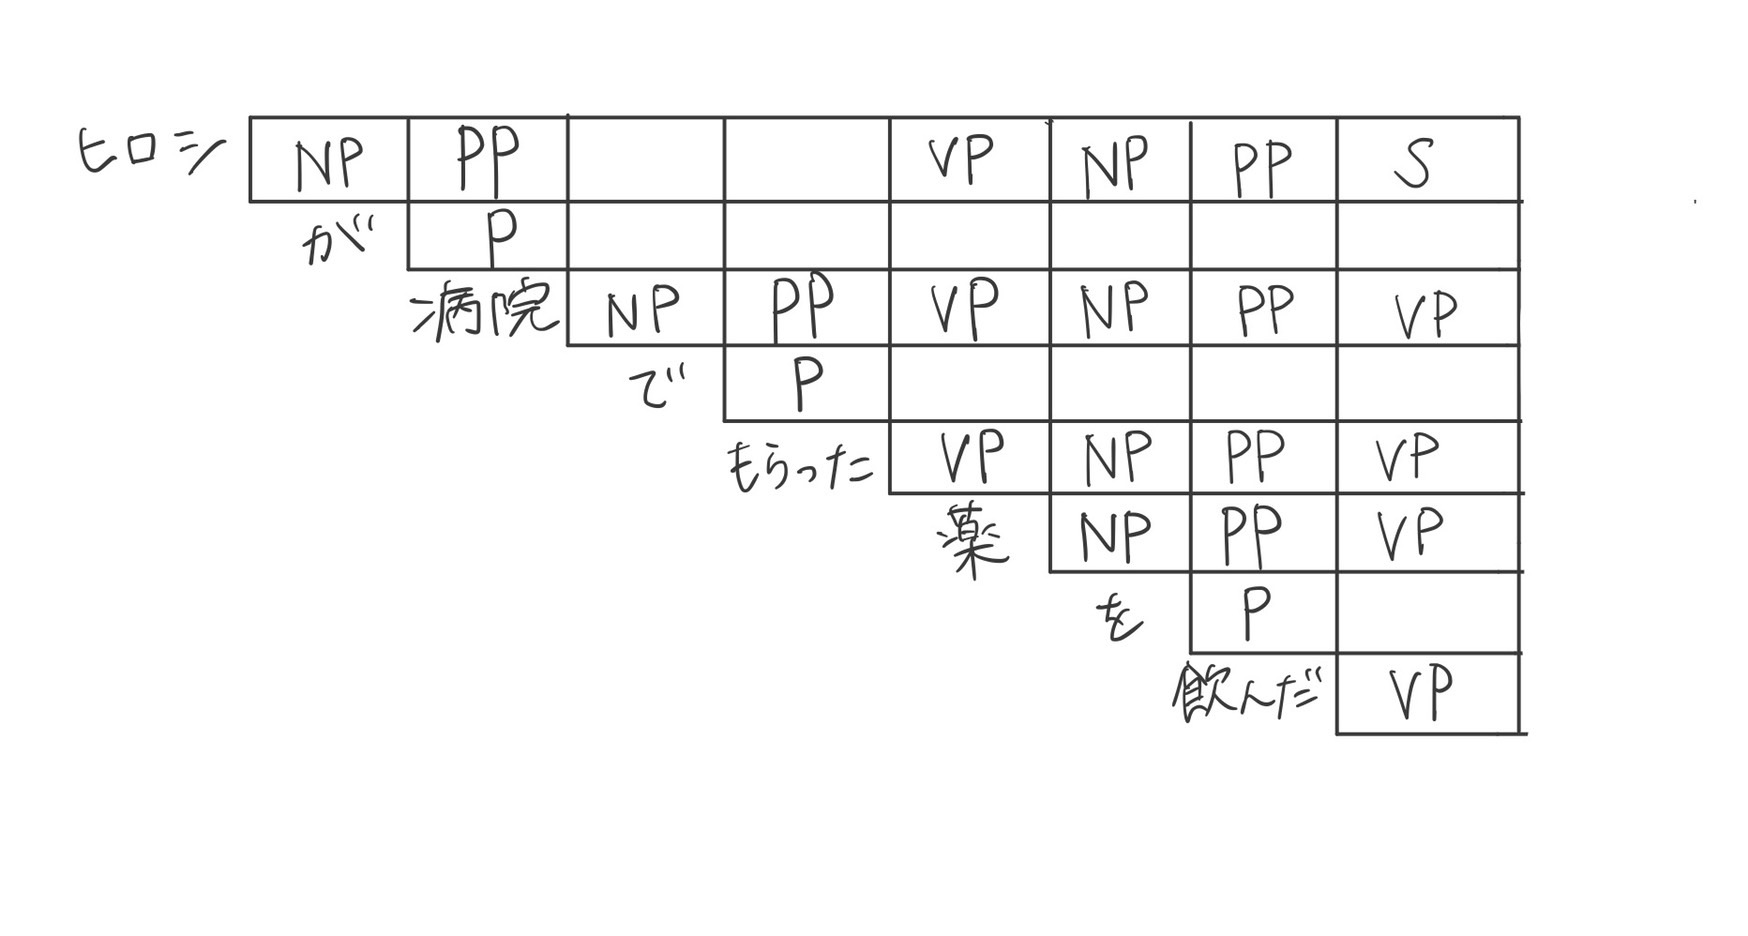
\includegraphics[scale=0.1]{s1.jpg}
    \caption{ラティス構造}\label{fig:図}
\end{figure}

\end{document}